\documentclass[a4paper]{article}
\usepackage[utf8]{inputenc}
\usepackage{amsmath} %untuk simbol matematika dasar
\usepackage{ulem}%untuk underline
\usepackage{graphicx}
\usepackage{geometry}
\geometry{left=2.5cm, right=2.5cm, top=3cm, bottom=3cm}
\usepackage[indonesian]{babel}
\usepackage{xcolor} % untuk text color

%definisi warna warna
\definecolor{vermilion}{RGB}{227,66,52}
\definecolor{amber}{RGB}{255,192,0}
\definecolor{chartreuse}{RGB}{128,255,0}
\definecolor{teal}{RGB}{0,128,128}
\definecolor{violet}{RGB}{128,0,255}
\definecolor{russet}{RGB}{128,70,27}
\definecolor{slate}{RGB}{112,128,144}
\definecolor{citron}{RGB}{221,208,106}
\definecolor{scarlet}{RGB}{255,36,0}
\definecolor{spring-green}{RGB}{0,255,128}
\definecolor{azure}{RGB}{0,128,255}
\definecolor{rose}{RGB}{255,0,128}

\usepackage{hyperref} % Untuk hyperlink
\usepackage{tocloft} % Untuk mengatur daftar isi dari suatu daftar (bukan table of content)

\usepackage{titling}
\usepackage{tikz} % untuk grafis dan pembuatan sampel warna
\usetikzlibrary{calc}

% Untuk mengubah format penomoran menjadi arab
\renewcommand\thesection{\arabic{section}}
% Untuk mengubah format penomoran agar mengabaikan label dari format penomoran section
\renewcommand\thesubsection{\arabic{section}.\arabic{subsection}}

% Untuk daftar pustaka pemformatan nomor dihapus
\newcommand{\nonumsection}[1]{\section*{#1}
\addcontentsline{toc}{section}{#1}
}

\usepackage{xparse} % flexible new command serta logical IfValueTF

\usepackage{mfirstuc} % kapital huruf pertama

% Membuat textbox dengan background warna tertentu
\NewDocumentCommand{\warnaln}{mo}{%
  \tikz[baseline=-0.5\ht\strutbox]{%
    \node[shape=rectangle, draw=black, fill=#1, minimum height=1.5em, inner sep=2pt]{%
      \IfValueTF{#2}{\capitalisewords{#2}}{
      \capitalisewords{#1}
      }%
    };
  }%
}

\newcommand{\warnalnbl}[1]{
  \tikz[baseline=-0.5\ht\strutbox]{
    \node[shape=rectangle, draw=black, fill=black, minimum height=1.5em, inner sep= 2pt, text=white]{#1}
  }
}

\title{
  \vspace{-3cm}
  \centering
  \vspace{1cm}
  \textbf{Teori Warna}\\
  \large Mata Kuliah: \textbf{Komunikasi Visual}
}
\author{$\begin{array}{c}
  \textbf{M Reza Dwi Prasetiawan}\\
  \textbf{Farhan Nur Fadilah}\\
  \textbf{Sigit Yulianto}\\
  \textbf{Shinta Ayu L}\\
  \textbf{Indah Lestari}\\
  \textbf{Agnes Nabila Putri}\\
  \textbf{Erni Rahmawati}\\
\end{array}$
}
\date{\today}

\begin{document}
\pagenumbering{gobble}
\begin{titlepage}
  \maketitle
  \vfill
  \begin{center}
    
\includegraphics[width=\textwidth]{resources/logo-univ.png}\\
    \large
    Teknologi Informasi\\
    Institut Teknologi dan Sains\\
    Nahdatul Ulama Lampung\\
    Dosen Pembimbing: \textbf{Dewi Puspitasari, M.Sos}
  \end{center}
\end{titlepage}

\newpage
\pagenumbering{arabic}
% Insert table of contents
\tableofcontents
\newpage

Dalam dunia desain grafis (\textit{graphic design}), warna menjadi komponen utama yang memegang peran penting dalam memikat target \textit{audience}, maupun untuk menggambarkan produk jika dalam desain \textit{branding}. Untuk memahami lebih jelasnya, di sini kami bagi menjadi 4 bab utama yaitu: Macam-macam warna, Psikologi warna, Skema warna, dan terakhir aplikasinya dalam dunia desain grafis.

\section{Macam-macam Warna}

Sebelum memahami bagaimana warna berpengaruh dalam psikologi, terlebih dahulu kita harus mengenal, apa saja sih jenis-jenis warna yang ada?

Umumnya warna dibagi menjadi 4 bagian: warna primer, warna sekunder, dan warna tersier (\textit{AKA} warna menengah atau \textit{intermediate}) dan terakhir warna kuaterner(namun tidak dibahas untuk memudahkan).
Warna primer adalah warna dasarnya, warna sekunder adalah gabungan dari dua warna primer dengan proporsi yang sama, sedangkan warna tersier adalah gabungan dari warna primer dan sekunder atau dua warna sekunder, yang terakhir warna kuaterner adalah kelompok warna dari perluasan warna tersier.

Ada beberapa model warna yang memiliki warna dasar yang berbeda-beda, yaitu model warna RYB (\warnaln{red}\warnaln{yellow}\warnaln{blue}), RGB (\warnaln{red}\warnaln{green}\warnaln{blue}), CMYK (\warnaln{cyan}\warnaln{magenta}\warnaln{yellow}\warnalnbl{Key/Black}), dan masih banyak lagi.

Terlepas dari model warna yang digunakan, ada juga warna komplementer dan warna netral yang disajikan setelah pembahasan model warna RYB, RGB, dan CMYK (model warna lain tidak akan dibahas di sini).

\subsection{Model Warna RYB}
\subsubsection{Warna Primer}
Dalam model warna RYB (\warnaln{red}\warnaln{yellow}\warnaln{blue}), warna dasar yang digunakan adalah merah, kuning, dan biru. Hal ini dikarenakan sistem RYB biasa digunakan untuk cat atau pigmen warna. Ketika cat/pigmen warna dicampurkan, hasilnya adalah pengurangan panjang gelombang cahaya yang dipantulkan. Oleh karena itu, model warna RYB disebut juga model warna substraktif.

\subsubsection{Warna Sekunder}
Karena model warna RYB hanya memiliki 3 warna dasar, maka warna sekundernya juga hanya ada 3, yaitu:
\begin{enumerate}
  \item \warnaln{orange}[oranye] = \warnaln{red}[merah] + \warnaln{yellow}[kuning]
  \item \warnaln{green}[hijau] = \warnaln{yellow}[kuning] + \warnaln{blue}[biru]
  \item \warnaln{purple}[ungu] = \warnaln{red}[merah] + \warnaln{blue}[biru]
\end{enumerate}

\subsubsection{Warna Tersier}
Seperti yang dijelaskan sebelumnya, warna tersier dihasilkan dari campuran dua warna primer-sekunder dan sekunder-sekunder.\\
Berikut warna-warnanya:
\begin{enumerate}
  \item \warnaln{vermilion}=\warnaln{red}[merah]+\warnaln{orange}[oranye]
  \item \warnaln{amber}=\warnaln{yellow}[kuning]+\warnaln{orange}[oranye]
  \item \warnaln{chartreuse}=\warnaln{yellow}[kuning]+\warnaln{green}[hijau]
  \item \warnaln{teal}=\warnaln{blue}[biru]+\warnaln{green}[hijau]
  \item \warnaln{violet}=\warnaln{purple}[ungu]+\warnaln{blue}[biru]
  \item \warnaln{magenta}=\warnaln{purple}[ungu]+\warnaln{red}[merah]
  \item \warnaln{russet}=\warnaln{orange}[oranye]+\warnaln{purple}[ungu]
  \item \warnaln{slate}=\warnaln{purple}[ungu]+\warnaln{green}[hijau]
  \item \warnaln{citron}=\warnaln{green}[hijau]+\warnaln{orange}[oranye]
\end{enumerate}

\subsection{Model Warna RGB}
\subsubsection{Warna primer}
Model warna ini adalah model warna additif karena menggunakan panjang gelombang cahaya sebagai prediksi warnanya. Model ini digunakan di dunia digital, karena warna dasar sejati adalah ini. Mata manusia memiliki 3 tipe reseptor cahaya yang masing masing mengenali warna \warnaln{red}[merah], \warnaln{green}[hijau] dan \warnaln{blue}[biru]. Di sisi lain warna netral \warnaln{white}[putih] dihasilkan dari saturasi penuh ketiganya, sedangkan warna netral \warnalnbl{Hitam} adalah ketiadaan saturasi di ketiganya

\subsubsection{Warna sekunder}
Berikut warna-warna sekundernya:
\begin{enumerate}
  \item \warnaln{yellow}[kuning]=\warnaln{red}[merah]+\warnaln{green}[hijau]
  \item \warnaln{cyan}=\warnaln{green}[hijau]+\warnaln{blue}[biru]
  \item \warnaln{magenta}=\warnaln{red}[merah]+\warnaln{blue}[biru]
\end{enumerate}

Dalam bentuk saturasi RGB menjadi:
\begin{enumerate}
  \item \warnaln{yellow}[Kuning]=\warnaln{red}[100\%]\warnaln{green}[100\%]\warnaln{blue}[0\%]
  \item \warnaln{cyan}=\warnaln{red}[0\%]\warnaln{green}[100\%]\warnaln{blue}[100\%]
  \item \warnaln{magenta}=\warnaln{red}[100\%]\warnaln{green}[0\%]\warnaln{blue}[100\%]
\end{enumerate}

\subsubsection{Warna Tersier}
Berikut warna-warna tersiernya langsung dalam bentuk saturasi RGB untuk memudahkan:
\begin{enumerate}
  \item \warnaln{orange}[oranye]=\warnaln{red}[100\%]\warnaln{green}[50\%]\warnaln{blue}[0\%]
  \item \warnaln{chartreuse}=\warnaln{red}[50\%]\warnaln{green}[100\%]\warnaln{blue}[0\%]
  \item \warnaln{spring-green}=\warnaln{red}[0\%]\warnaln{green}[100\%]\warnaln{blue}[50\%]
  \item \warnaln{azure}=\warnaln{red}[0\%]\warnaln{green}[50\%]\warnaln{blue}[100\%]
  \item \warnaln{violet}=\warnaln{red}[50\%]\warnaln{green}[0\%]\warnaln{blue}[100\%]
  \item \warnaln{rose}=\warnaln{red}[100\%]\warnaln{green}[0\%]\warnaln{blue}[50\%]
\end{enumerate}

\subsection{Model Warna CMYK}
\subsubsection{Warna primer}
Model warna ini sama dengan model warna RYB yaitu model warna substraktif. Perbedaannya terletak pada warna dasarnya, yaitu \warnaln{cyan}, \warnaln{magenta}, \warnaln{yellow} dan \warnalnbl{Key/Black} sebagai pengatur kecerahannya. Model ini dibuat sebagai respon atas susah mencetak (\textit{print}) kertas sama persis seperti \textit{input}nya(misalnya gambar atau dokumen seperti \textit{pdf}). Model ini substraktif karena cara kerjanya adalah dengan mengurangi panjang gelombang cahaya putih(dari \textit{background}nya) yang dipantulkannya ke mata.

\subsubsection{Warna sekunder}
Karena warna \warnalnbl{Hitam} hanyalah berperan sebagai \textit{key} atau kunci yang mengatur kecerahannya, warna warna sekundernya pada dasarnya juga 3 yang sama persis dengan warna dasar model warna RGB.\\ Berikut warna-warnanya:
\begin{enumerate}
  \item \warnaln{red}[merah]=\warnaln{magenta}+\warnaln{yellow}[kuning]
  \item \warnaln{green}[hijau]=\warnaln{cyan}+\warnaln{yellow}[kuning]
  \item \warnaln{blue}[biru]=\warnaln{cyan}+\warnaln{magenta}
\end{enumerate}

\subsubsection{Warna tersier}
Warna tersiernya sama persis dengan warna tersier RGB\\
berikut warna-warnanya dan warna-warna yang membentuknya:
\begin{enumerate}
  \item \warnaln{orange}[oranye]=\warnaln{red}[merah]+\warnaln{yellow}[kuning]
  \item \warnaln{chartreuse}=\warnaln{yellow}[kuning]+\warnaln{green}[hijau]
  \item \warnaln{spring-green}=\warnaln{green}+\warnaln{cyan}
  \item \warnaln{azure}=\warnaln{cyan}+\warnaln{blue}
  \item \warnaln{violet}=\warnaln{blue}[biru]+\warnaln{magenta}
  \item \warnaln{rose}=\warnaln{red}[merah]+\warnaln{magenta}
\end{enumerate}

\subsection{Warna Komplementer}
Warna komplementer bukanlah satu warna, melainkan dua warna yang saling berlawanan kontras. Berikut ciri-cirinya:
\begin{enumerate}
  \item Kontrasnya saling berlawanan
  \item Terdiri dari satu warna hangat dan satu warna dingin
  \item Ketika diletakkan berdampingan, menciptakan kontras yang kuat
\end{enumerate}

Berikut beberapa contoh warna komplementer:
\begin{itemize}
  \item \warnaln{red}[merah] \warnaln{green}[hijau]
  \item \warnaln{blue}[biru] \warnaln{orange}[oranye]
  \item \warnaln{yellow}[kuning] \warnaln{purple}[ungu]
\end{itemize}

\subsection{Warna Netral}
Warna netral tidak memiliki nuansa tertentu dan biasa digunakan sebagai latar belakang (\textit{background}) dari suatu desain, atau justru digabungkan dengan warna lain untuk menyeimbangkan warna-warna lainnya. Ada empat warna netral utama yaitu \warnalnbl{Hitam}, \warnaln{white}[putih], \warnaln{brown}[coklat], dan \warnaln{gray}[abu-abu]. Warna netral biasanya dihasilkan dari dua warna yang saling berlawanan (warna komplementer).

\section{Psikologi Warna}
Sebelumnya kita telah mengetahui macam-macam warna dari beberapa model warna, sekarang kami akan menyajikan, apa sih Psikologi warna itu? dan bagaimana warna berpengaruh terhadap psikologi pengamat?
\subsection{Pengertian Psikologi Warna}
Berdasarkan \textit{\textbf{KBBI} Psikologi} adalah:
\begin{enumerate}
  \item ilmu yang berkaitan dengan proses mental, baik normal maupun abnormal dan pengaruhnya pada perilaku
  \item ilmu pengetahuan tentang gejala dan kegiatan jiwa
\end{enumerate}
Sedangkan \textit{warna} adalah:
\begin{enumerate}
  \item kesan yang diperoleh mata dari cahaya yang dipantulkan oleh benda-benda yang dikenainya;
  \item corak rupa, seperti biru dan hijau: dia sering memakai baju yang biru --nya
  \item kl kasta; golongan; tingkatan (dalam masyarakat): masyarakat Hindu membagi manusia menjadi empat --
  \item kl corak; ragam (sifat sesuatu): usaha partai itu tidak jelas --nya
\end{enumerate}

Namun untuk warna dalam konteks ini, definisi yang sesuai hanya 1 dan 2. Sehingga dapat disimpulkan bahwa \underline{Psikologi warna} adalah ilmu yang mempelajari tentang pengaruh suatu corak rupa(dalam hal ini \textit{warna}) terhadap perasaan, perilaku, dan persepsi pengamat.
Berikut beberapa aspek penting tentang psikologi warna

\subsection{Asosiasi warna}
Warna memiliki dampak yang signifikan terhadap emosi, persepsi, dan perilaku manusia. Dalam banyak konteks budaya, warna sering kali diasosiasikan dengan berbagai sifat, makna, dan perasaan tertentu. Berikut adalah beberapa asosiasi warna yang umum, yang masing-masing mewakili berbagai aspek kehidupan manusia:
\begin{enumerate}
  \item \warnaln{red}[merah] $\implies$ Warna merah sering kali dikaitkan dengan energi yang tinggi, gairah, dan intensitas. Ini adalah warna yang memicu respons emosional yang kuat, sering dihubungkan dengan cinta dan agresi. Warna merah juga melambangkan bahaya, peringatan, atau kekuatan yang mendesak. Dalam konteks positif, merah dapat membangkitkan semangat dan keinginan yang kuat, tetapi dalam konteks negatif, merah juga dapat diasosiasikan dengan amarah dan konflik. Di banyak budaya, warna merah juga merupakan simbol dari keberuntungan atau kebahagiaan, seperti di China di mana merah melambangkan kebahagiaan dalam pernikahan dan perayaan lainnya.
  \item \warnaln{blue}[biru] $\implies$ Biru sering dianggap sebagai warna yang menenangkan dan membawa kedamaian. Ini adalah warna yang melambangkan ketenangan, kepercayaan, dan stabilitas. Warna biru sering digunakan dalam lingkungan kerja profesional karena dapat menumbuhkan rasa kepercayaan dan kredibilitas. Dalam psikologi warna, biru juga dikenal dapat mengurangi kecemasan dan memberikan efek menenangkan yang membantu seseorang berkonsentrasi lebih baik. Karena asosiasinya dengan laut dan langit, biru juga sering dikaitkan dengan kebebasan dan ketidakberhinggaan.
  \item \warnaln{green}[Hijau] $\implies$ Warna hijau sering dihubungkan dengan alam dan pertumbuhan. Ini adalah warna yang mewakili keseimbangan, harmoni, dan ketenangan. Hijau juga dapat melambangkan kesegaran, kesehatan, dan vitalitas. Dalam konteks lingkungan, hijau adalah simbol dari konservasi dan keberlanjutan. Penggunaan hijau dalam desain sering dimaksudkan untuk memberikan efek menenangkan, sehingga banyak digunakan di ruang-ruang yang berfungsi untuk relaksasi dan pemulihan. Selain itu, hijau juga diasosiasikan dengan keberuntungan, seperti dalam budaya Barat di mana hijau melambangkan nasib baik dan kelimpahan.
  \item \warnaln{yellow}[Kuning] Kuning adalah warna yang penuh energi dan optimisme. Ini adalah warna yang melambangkan kebahagiaan, kreativitas, dan kecerdasan. Kuning sering dikaitkan dengan sinar matahari, yang dapat memberikan perasaan hangat dan cerah. Warna ini dapat merangsang mental dan meningkatkan aktivitas otak, oleh karena itu sering digunakan dalam konteks yang membutuhkan stimulasi intelektual atau kreativitas. Namun, penggunaan kuning yang berlebihan juga dapat menimbulkan perasaan gelisah atau kecemasan, karena warna ini sangat kuat dan mencolok.
  \item \warnaln{purple}[ungu] $\implies$ Ungu adalah warna yang sering diasosiasikan dengan kemewahan, spiritualitas, dan misteri. Dalam sejarah, warna ungu sering dikaitkan dengan kerajaan dan kebangsawanan, karena pigmen ungu dahulu sangat langka dan mahal. Selain itu, ungu juga memiliki konotasi spiritual yang mendalam, sering dikaitkan dengan kebijaksanaan dan meditasi. Ungu juga dapat merangsang imajinasi dan kreativitas, sehingga sering digunakan dalam konteks seni dan desain. Warna ini membawa perasaan introspektif dan reflektif yang dapat meningkatkan intuisi.
  \item \warnalnbl{Hitam} $\implies$ Warna hitam sering kali diasosiasikan dengan kekuatan, keanggunan, dan misteri. Di satu sisi, hitam adalah warna yang melambangkan formalitas dan keanggunan, sering digunakan dalam mode dan desain untuk memberikan kesan mewah. Di sisi lain, hitam juga memiliki asosiasi dengan kesedihan dan kematian, menjadikannya simbol dari keseriusan dan tragedi. Hitam juga merupakan warna yang digunakan untuk menunjukkan kekuatan dan kontrol, sehingga banyak digunakan dalam situasi di mana otoritas perlu ditegaskan. Dalam konteks psikologi warna, hitam juga dapat melambangkan perlindungan dan isolasi.
  \item \warnaln{white}[putih] $\implies$ Putih melambangkan kemurnian, kesucian, dan kebersihan. Ini adalah warna yang sering digunakan dalam konteks yang membutuhkan ketulusan dan kesederhanaan. Dalam banyak budaya, putih adalah simbol dari awal yang baru atau kebersihan spiritual, sering kali digunakan dalam upacara pernikahan atau ritual keagamaan. Warna putih juga diasosiasikan dengan kesederhanaan dan minimalisme, digunakan dalam desain untuk menciptakan ruang yang terbuka dan bersih. Di sisi lain, putih juga dapat melambangkan kerapuhan atau kehampaan.
\end{enumerate}

\subsection{Faktor-faktor yang Mempengaruhi Persepsi Warna}
Faktor-faktor yang mempengaruhi persepsi warna sangat bervariasi dan kompleks. Persepsi warna tidak hanya ditentukan oleh kualitas fisik warna itu sendiri, tetapi juga oleh berbagai faktor lain yang memengaruhi bagaimana seseorang merasakan dan menafsirkan warna tertentu. Berikut adalah beberapa faktor utama yang dapat memengaruhi persepsi warna seseorang:

\subsubsection{Budaya}
Makna warna dapat sangat bervariasi di berbagai budaya. Setiap budaya memiliki interpretasi dan asosiasi unik terhadap warna tertentu. Misalnya, warna putih yang sering diasosiasikan dengan kemurnian atau pernikahan di budaya Barat, justru diasosiasikan dengan duka dan kematian di beberapa budaya Asia, seperti di China dan India. Warna merah di Barat sering dikaitkan dengan cinta dan gairah, sementara di China, merah adalah simbol keberuntungan dan kebahagiaan. Oleh karena itu, konteks budaya memainkan peran penting dalam bagaimana seseorang menafsirkan warna tertentu.


\subsubsection{Usia}
Persepsi warna dapat berubah seiring bertambahnya usia. Pada usia muda, mata manusia umumnya dapat menangkap spektrum warna dengan jelas dan tajam. Namun, seiring bertambahnya usia, kemampuan mata untuk mendeteksi warna bisa menurun. Hal ini terjadi karena lensa mata menjadi lebih kuning dan buram, sehingga mengurangi sensitivitas terhadap warna-warna cerah, terutama pada spektrum biru dan hijau. Orang yang lebih tua mungkin juga melihat warna dengan intensitas yang lebih rendah dibandingkan orang yang lebih muda. Hal ini dapat mempengaruhi preferensi warna dan cara seseorang merespons warna-warna tertentu.


\subsubsection{Jenis Kelamin} Jenis kelamin juga mempengaruhi persepsi warna. Penelitian menunjukkan bahwa perempuan cenderung lebih sensitif terhadap warna daripada laki-laki. Perempuan umumnya lebih mampu membedakan antara nuansa warna yang berbeda, terutama dalam spektrum merah dan oranye. Sementara itu, laki-laki cenderung memiliki kemampuan yang lebih terbatas dalam membedakan variasi warna yang halus. Selain itu, dalam beberapa kasus, laki-laki lebih mungkin mengalami buta warna, khususnya buta warna merah-hijau, yang juga dapat mempengaruhi bagaimana mereka melihat dunia di sekitar mereka.


\subsubsection{Pengalaman Pribadi}
Pengalaman pribadi juga sangat berpengaruh terhadap persepsi warna seseorang. Warna tertentu dapat memicu ingatan, perasaan, atau asosiasi yang kuat berdasarkan pengalaman masa lalu. Misalnya, seseorang yang memiliki kenangan indah yang terkait dengan warna biru mungkin merasa tenang atau bahagia ketika melihat warna biru. Sebaliknya, warna tertentu juga dapat membawa ingatan yang negatif atau traumatis. Misalnya, warna merah bisa menimbulkan kecemasan bagi seseorang yang pernah mengalami pengalaman berbahaya atau menakutkan yang melibatkan warna tersebut. Pengalaman visual seseorang terhadap lingkungan tempat tinggal, pendidikan, dan interaksi sosial juga dapat memengaruhi bagaimana mereka memaknai warna.

\newpage

\section{Skema Warna}
Skema warna terdiri dari kombinasi warna yang digunakan dalam berbagai disiplin ilmu desain, dari seni rupa hingga desain interior hingga desain grafis. Setiap skema warna terdiri dari satu atau lebih dari dua belas warna yang ada pada roda warna. Dengan memasangkan warna yang berbeda satu sama lain, Anda dapat membuat palet warna tanpa akhir untuk digunakan dalam komposisi apa pun. Kombinasi warna yang berbeda membangkitkan suasana hati atau nada yang berbeda dengan menggunakan teori warna dan psikologi warna.

\subsection{Skema Warna Monokromatik}
\begin{center}
  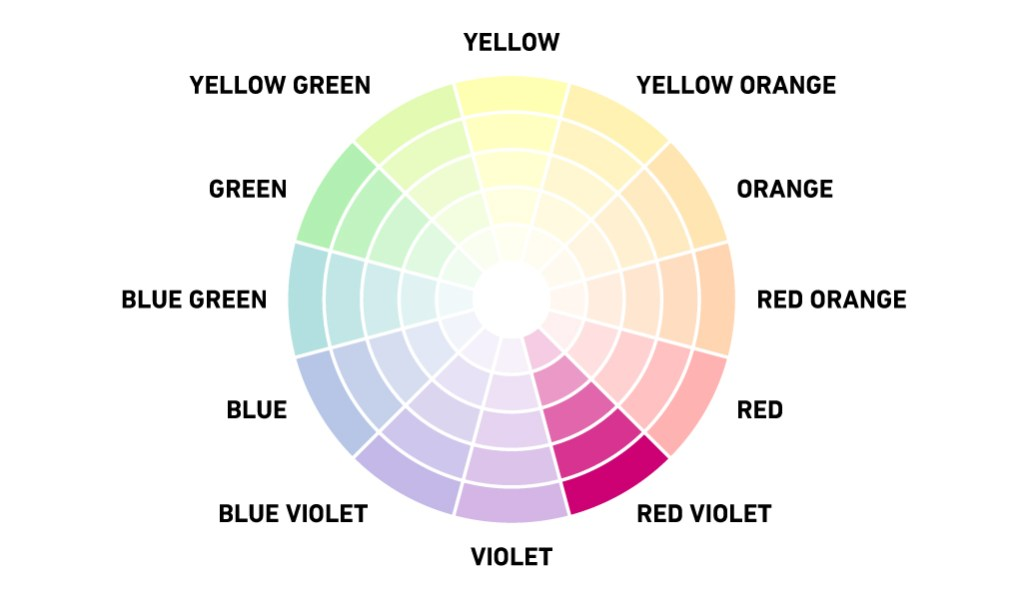
\includegraphics[width=\widthtext]{resources/monochromatic.jpg}
\end{center}
Skema warna monokromatik berfokus pada satu warna, sering kali menggunakan variasi rona tersebut dengan menggabungkan rona, nada, dan corak. Dengan menambahkan sedikit warna putih, abu-abu, atau hitam, warna tunggal itu berkembang menjadi seluruh palet dengan jumlah nilai yang bervariasi. Tint, tone, dan shade tersebut memberikan highlight dan bayangan untuk merapikan palet warna yang datar.

Skema warna ini sangat fleksibel dan mudah dilihat. Menggunakan banyak rona dalam sebuah desain sering kali dapat menyebabkan bentrokan warna dan menghalangi tampilan desain; variasi warna yang kontras pada satu rona membantu menyederhanakan desain tanpa membuatnya terlalu datar. Dalam ilustrasi di bawah ini, penggabungan warna oranye dan coklat yang lebih gelap memberikan ketertarikan visual sambil tetap menjaga skema warna keseluruhan tetap minimal.

Skema warna monokromatik juga semakin populer karena munculnya minimalis di semua aspek desain, mulai dari desain interior hingga desain kemasan hingga desain situs web. Skema warna ini juga menyediakan ruang yang cukup untuk konten atau informasi penting di situs web atau iklan.

\subsection{Skema Warna Pelengkap}
\begin{center}
  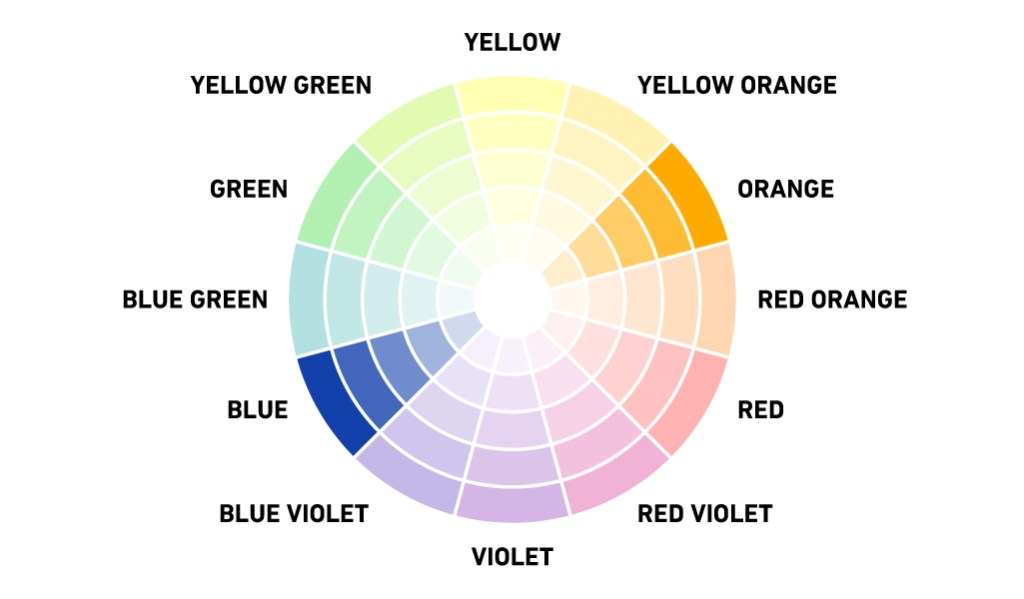
\includegraphics[width=\widthtext]{resources/pelengkap.jpg}
\end{center}
Warna komplementer ada di sisi berlawanan dari roda warna; satu warna biasanya merupakan warna primer dan yang lainnya merupakan warna sekunder. Warna pelengkap utama biasanya biru dan oranye, merah dan hijau, dan kuning dan ungu.

Warna yang berlawanan satu sama lain pada roda warna biasanya memberikan kontras tinggi saat dipasangkan bersama. Pada saturasi penuh, rona komplementer bisa terlalu intens untuk pemirsa. Untuk mengurangi intensitas, gabungkan tint, tone, dan shade untuk memperluas palet, seperti yang kita lakukan dengan skema warna monokromatik. Misalnya, desain merek Rico Rico di bawah ini menggabungkan nilai oranye dan biru yang lebih terang dan lebih gelap untuk membuat palet pelengkap lebih mudah dilihat.

Ketika dilakukan dengan sukses, palet pelengkap dapat membuat dampak besar pada desain. Pasangan rona hangat dan dingin memberikan kontras yang kaya dan menarik. Pada awalnya, menggunakan skema yang saling melengkapi bisa sangat melelahkan; merangkul trial and error dan bereksperimen dengan berbagai palet. Untuk panduan warna, gunakan alat praktis ini untuk menyusun palet warna Anda berikutnya.
\subsection{Skema Warna Analog}
Warna analog terdiri dari sekelompok tiga warna yang berbatasan satu sama lain dalam roda warna. Skema warna ini dimulai dengan rona dasar dan diperluas dengan dua rona tetangga. Kata "analog" berarti terkait erat, sehingga kombinasi warna ini memiliki daya tarik yang harmonis mirip dengan skema warna monokromatik.

Palet ini dikenal menyenangkan mata, jadi jika Anda tidak yakin skema warna mana yang akan digunakan dalam proyek Anda berikutnya, palet warna analog tidak pernah mengecewakan. Saat memilih grup analog untuk proyek Anda, jaga agar palet Anda tetap membumi dengan menggunakan warna-warna dingin atau hangat secara eksklusif bersama-sama.

Jika Anda membutuhkan inspirasi warna, lihatlah di sekitar Anda. Palet analog secara rutin ditemukan di alam, dari matahari terbenam yang indah hingga bulu burung yang memikat hingga lautan yang menawan, memberi Anda perasaan tenang dan damai. Misalnya, desain kartu nama untuk Talkfest di atas menggabungkan warna merah, merah muda, dan oranye, memberikan desain kualitas matahari terbenam.

\subsection{Skema Warna Triadik}
\begin{center}
  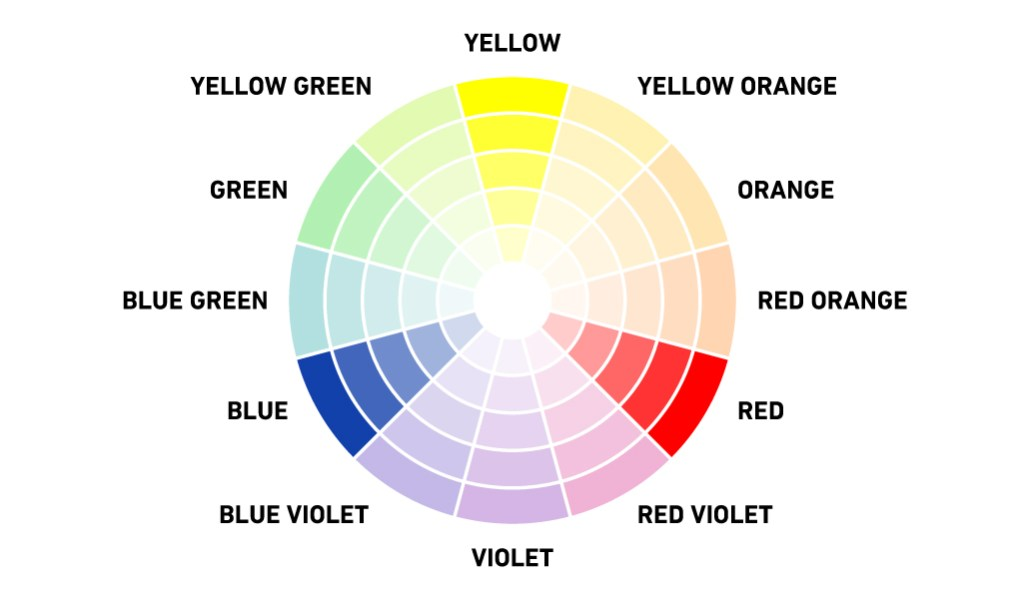
\includegraphics[width=\widthtext]{resources/triadic.jpg}
\end{center}
Sebuah triad terdiri dari tiga warna yang ditempatkan pada jarak yang sama satu sama lain pada roda warna, membentuk segitiga seperti yang terlihat di bawah ini. Skema warna triadik dapat mencakup tiga warna primer, sekunder, atau tersier. Palet triadik umum terdiri dari biru, merah, dan kuning atau ungu, hijau, dan oranye.

Kebanyakan palet triadik berwarna cerah dan sulit untuk diseimbangkan. Tetapkan satu rona dasar, lalu gunakan rona yang tersisa sebagai warna aksen. Ketika semua warna dalam skema triadik digunakan secara merata, setiap rona sering memperebutkan sorotan. Cara yang baik untuk mencegah bentrokan warna adalah dengan menetapkan hierarki warna dalam komposisi.

Seperti skema warna lainnya, hindari menggunakan ketiga rona dalam keadaan jenuh penuh. Bawa sedikit warna putih, abu-abu, atau hitam untuk mengurangi warna dan memperluas palet.

\subsection{Skema Warna Netral}
\begin{center}
  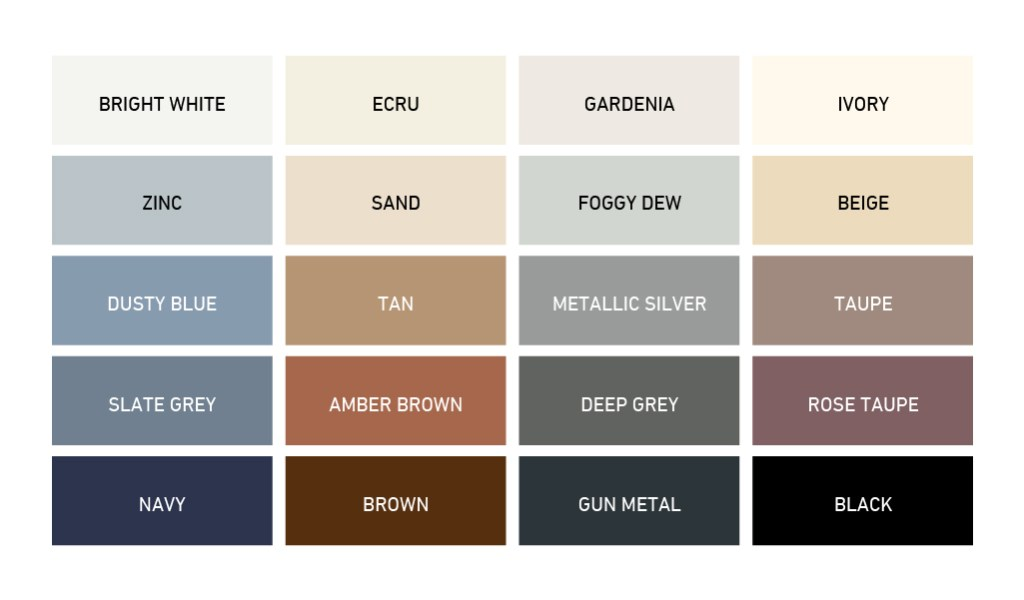
\includegraphics[width=\widthtext]{resources/netral.jpg}
\end{center}
Palet warna netral baru-baru ini mendapatkan momentum di semua disiplin desain. Skema warna yang populer biasanya terdiri dari rona akromatik (putih, abu-abu, dan hitam) bersama dengan hampir netral (krem, cokelat, coklat, dan warna gelap lainnya). Semua warna netral memiliki satu kesamaan: mereka biasanya desaturasi dengan bantuan tint, tone, dan shade.

Skema warna ini dapat disesuaikan dengan berbagai aplikasi dan media; estetika netral telah menemukan tempatnya di antara desain merek, alat tulis, dekorasi interior, dan di media sosial. Keindahan skema warna ini adalah sulit untuk berlebihan dengan warna, tetapi sebagai aturan praktis, cobalah tetap berpegang pada empat warna atau kurang.

Sama seperti skema warna monokromatik, palet netral membangkitkan rasa ketenangan dan ketenangan. Nada desaturasi mudah dilihat dan tidak sesuai dengan tren tertentu.

\section{Aplikasi Warna Dalam Desain}
Warna memegang peranan penting dalam desain, tidak hanya sebagai elemen visual, tetapi juga sebagai alat komunikasi yang kuat untuk memengaruhi perasaan, emosi, dan persepsi audiens. Pemilihan warna yang tepat dalam desain dapat memperkuat pesan, menciptakan suasana yang diinginkan, dan bahkan memengaruhi perilaku pengguna. Berikut adalah beberapa prinsip dan aplikasi penggunaan warna dalam desain berdasarkan faktor-faktor yang mempengaruhi persepsi warna:

\subsubsection{Pemilihan Warna Berdasarkan Budaya}
Ketika merancang untuk audiens global atau budaya tertentu, desainer harus memahami bagaimana warna diterima dalam budaya tersebut. Misalnya, warna merah mungkin tepat untuk menarik perhatian di situs web yang berfokus pada keberuntungan di budaya China, tetapi mungkin tidak cocok di negara-negara Barat untuk tema yang sama. Oleh karena itu, pengetahuan mendalam tentang asosiasi warna dalam budaya audiens sangat penting untuk memastikan pesan yang disampaikan tidak disalahpahami atau dianggap negatif. Untuk kampanye internasional, pemilihan warna yang netral atau universal, seperti biru, sering digunakan karena cenderung diterima secara positif di banyak budaya sebagai simbol stabilitas dan kepercayaan.

\subsubsection{Penggunaan Warna yang Tepat Berdasarkan Usia}
Usia audiens juga harus menjadi pertimbangan utama dalam pemilihan warna. Desain untuk anak-anak sering kali menggunakan warna-warna cerah dan kontras yang dapat dengan mudah menarik perhatian, seperti merah, kuning, dan hijau cerah. Anak-anak merespons warna yang kuat dan cerah secara lebih antusias dibandingkan dengan warna-warna yang lembut. Sebaliknya, desain untuk orang dewasa yang lebih tua mungkin perlu memperhatikan bahwa kemampuan mereka untuk melihat warna, terutama warna seperti biru, mulai berkurang seiring usia. Oleh karena itu, penggunaan warna-warna yang lebih hangat dan kontras yang cukup tinggi mungkin lebih efektif untuk kelompok usia ini, sekaligus menghindari warna yang terlalu lembut atau dingin.


\subsection{Desain Berdasarkan Jenis Kelamin}
Mengingat adanya perbedaan dalam persepsi warna antara laki-laki dan perempuan, beberapa desain produk atau antarmuka dapat mempertimbangkan preferensi yang sering ditemui pada masing-masing jenis kelamin. Misalnya, studi menunjukkan bahwa perempuan cenderung lebih menyukai nuansa warna yang lebih halus dan beragam, seperti variasi pastel atau warna-warna dengan spektrum merah muda, sementara laki-laki mungkin lebih menyukai warna-warna yang kuat dan sederhana seperti biru atau abu-abu. Namun, penting untuk dicatat bahwa preferensi ini tidak universal, dan tren desain modern cenderung lebih inklusif, dengan warna-warna netral gender yang semakin populer untuk menciptakan daya tarik yang lebih luas.


\subsection{Pengalaman Pribadi dalam Pemilihan Warna}
Warna dalam desain dapat digunakan untuk memicu emosi atau kenangan yang terkait dengan pengalaman pribadi seseorang. Sebuah desain yang menampilkan warna-warna alam seperti hijau dan biru mungkin memberikan kesan ketenangan atau keseimbangan, karena banyak orang mengasosiasikan warna-warna ini dengan alam dan relaksasi. Di sisi lain, warna yang lebih hangat seperti oranye atau merah dapat menciptakan perasaan kegembiraan atau urgensi. Desainer dapat memanfaatkan kekuatan emosional warna ini untuk menciptakan pengalaman pengguna yang lebih dalam. Dalam pemasaran, misalnya, warna merah sering digunakan untuk tombol call-to-action (CTA) karena sifatnya yang menarik perhatian dan memberikan rasa urgensi.


\subsection{Menggunakan Kontras untuk Aksesibilitas}
Selain makna psikologis, pemilihan warna juga harus memperhatikan aksesibilitas. Desain yang inklusif perlu mempertimbangkan pengguna dengan gangguan penglihatan atau buta warna. Menggunakan kontras warna yang cukup antara teks dan latar belakang sangat penting untuk memastikan keterbacaan, terutama di platform digital. Misalnya, teks putih pada latar belakang hitam memberikan kontras yang tinggi dan mudah dibaca. Desainer juga dapat menggunakan alat bantu aksesibilitas, seperti color contrast checkers, untuk memastikan desain mereka dapat diakses oleh semua orang.


\subsection{Menyesuaikan Warna untuk Branding dan Identitas Visual}
Warna sering kali menjadi elemen inti dari identitas visual sebuah merek. Warna yang dipilih untuk branding harus konsisten dengan nilai dan pesan yang ingin disampaikan oleh merek tersebut. Misalnya, banyak perusahaan teknologi menggunakan warna biru untuk menonjolkan stabilitas, kepercayaan, dan profesionalitas. Di sisi lain, merek yang ingin menonjolkan kreativitas dan energi, seperti perusahaan fashion atau hiburan, mungkin menggunakan warna-warna cerah seperti merah atau kuning. Konsistensi penggunaan warna di berbagai media, seperti logo, situs web, dan materi pemasaran, dapat memperkuat identitas merek dan meningkatkan pengenalan merek oleh konsumen.


\subsection{Menciptakan Suasana melalui Skema Warna}
Pemilihan skema warna yang sesuai dapat membantu menciptakan suasana yang diinginkan dalam desain. Warna-warna sejuk seperti biru dan hijau cenderung menciptakan suasana yang tenang dan damai, cocok untuk desain interior rumah sakit atau spa. Sebaliknya, warna-warna hangat seperti merah dan oranye menciptakan suasana yang hangat, energik, dan penuh semangat, sehingga sering digunakan dalam desain restoran atau ruang publik yang menginginkan suasana yang dinamis. Pemilihan skema warna yang harmonis juga dapat memengaruhi cara audiens berinteraksi dengan ruang atau produk, sehingga penting bagi desainer untuk memilih skema warna yang tepat sesuai dengan tujuan desain.


\newpage
\nonumsection{Daftar Pustaka}
\begin{enumerate}
  \item \textcolor{blue}{\href{https://thecolorsmeaning.com/tertiary-colors/}{The Color Meaning - Tertiary Colors}}
  \item \textcolor{blue}{\href{https://medium.com/a-history-of-color/neutral-colors-e394cfce452}{Medium - Neutral Colors by Erin S}}
  \item \textcolor{blue}{\href{https://en.m.wikipedia.org/wiki/Color_scheme}{Wikipedia - Color Scheme}}
  \item \textcolor{blue}{\href{https://en.m.wikipedia.org/wiki/Secondary_color}{Wikipedia - Secondary colors}}
  \item \textcolor{blue}{\href{https://en.m.wikipedia.org/wiki/RGB_color_model}{Wikipedia - RGB color model}}
  \item \textcolor{blue}{\href{https://en.m.wikipedia.org/wiki/CMYK_color_model}{Wikipedia - CMYK color model}}
  \item \textcolor{blue}{\href{https://en.m.wikipedia.org/wiki/Vermilion}{Wikipedia - Vermilion}}
  \item \textcolor{blue}{\href{https://en.m.wikipedia.org/wiki/Amber_(color)}{Wikipedia - Amber}}
  \item \textcolor{blue}{\href{https://en.m.wikipedia.org/wiki/Chartreuse_(color)}{Wikipedia - Chartreuse}}
  \item \textcolor{blue}{\href{https://en.m.wikipedia.org/wiki/Teal}{Wikipedia - Teal}}
  \item \textcolor{blue}{\href{https://en.m.wikipedia.org/wiki/Russet_(color)}{Wikipedia - Russet}}
  \item \textcolor{blue}{\href{https://en.m.wikipedia.org/wiki/Slate_gray}{Wikipedia - Slate gray}}
  \item \textcolor{blue}{\href{https://en.m.wikipedia.org/wiki/Citron_(color)}{Wikipedia - Citron}}
  \item \textcolor{blue}{\href{https://en.m.wikipedia.org/wiki/Violet_(color)}{Wikipedia - Violet}}
  \item \textcolor{blue}{\href{https://kbbi.kemdikbud.go.id/entri/Warna}{KBBI - warna}}
  \item \textcolor{blue}{\href{https://kbbi.kemdikbud.go.id/entri/Psikologi}{KBBI - Psikologi}}
  
\end{enumerate}
\end{document}